\documentclass[../ZF_Wing.tex]{subfiles}
\begin{document}

\paragraph{Überblick Rechnungswesen}

Rechnungswesen = FIBU und BEBU\\
FIBU/Externe Rechnungswesen(Aufwände und Erträge) = Bilanz, Erfolgsrechnung,Geldflussrechnung\\
BEBU/Interne Rechnungswesen (Kosten und Leistungen) = Vollkostenrechnung, Teilkostenrechnung, Kalkulation\\

\textbf{Ziel BEBU:} Überwachung der Wirtschaftlichkeit der betrieblichen\\ Leistungserstellung und Leistungsveräusserung. Grundlage der Kalkulation. \\

Hat 3 Bereiche:
\begin{enumerate}
	\item Kostenarten
	\begin{itemize}
		\item Welche Kosten fallen an?
	\end{itemize}
	\item Kostenstellen
	\begin{itemize}
		\item Wo fallen Kosten an?
	\end{itemize}
	\item Kostenträgern
	\begin{itemize}
		\item Wofür fallen Kosten an?
	\end{itemize}
	\item Zuschlagsätze
\end{enumerate}


\paragraph{Gesamtheit der Kosten (Sume der Kostenarten nach Abgrenzung)\\}
\textbf{Direkt:} Einzelkosten
\textbf{Indirekt:} Gemein-Kosten


\subsection{Vollkostenrechnung}
Rückwirkend oder als Planung.\\
\paragraph{Hauptaufgaben:\\}
\begin{itemize}
	\item Dispositionsfunktion
	\begin{itemize}
		\item Ermittlung Selbstkosten
		\item Ermittlung Rechnungsgrundlagen für Programm-Verfahrensentscheidungen
		\item Ermittlung Bilanzansätzen		
	\end{itemize}
	\item Vorgabefunktion
	\begin{itemize}
		\item Vorgabe Sollkosten (auf Grundlage von Ist-,Normal-und/oder Plankosten)
	\end{itemize}
	\item Überwachungsfunktion
	\begin{itemize}
		\item Kurzfriste Erfolgsermittlung
		\item Wirtschaftlichkeitskontrolle
		\item Planabweichungsanalyse / Soll-Ist-Vergleiche
	\end{itemize}
\end{itemize}

\subsubsection{Beispiele Sachliche Abgrenzungen}
\begin{itemize}
	\item Kalkulatorische Zinsen
	\begin{itemize}
		\item Berücksichtigt, dass eigentlich auf dem EK auch ein Zins bezahlt weren müsste = Oppurtinitätskosten!
	\end{itemize}		
		\item Kalkulatorischer Unternehmerlohn 
		\begin{itemize}
			\item fiktives Gehalt des Unternehmers			
		\end{itemize}
		\item Kalkulatorische Miete
		\begin{itemize}
			\item fiktive Miete für die Benutzung eigener Räumlichkeien des Unternehmens = Oppurtunitätskosten!
		\end{itemize}
		\item Stille Reserven
		\begin{itemize}
			\item Über-/Unterbewertung Anlagevermögen, Lager
		\end{itemize}
		\item Kalkulatorische Abschreibungen
		\begin{itemize}
			\item Abweichender Abschreibungsaufwand FIBU/BEBU
		\end{itemize}
\end{itemize}


\subsubsection{Aufgaben der Kostenstellenrechnung}
\begin{itemize}
	\item Verteilung Kostenarten (Gemeinkosten) auf Kostenstellen
	\item Umlage von Kostenstellenkosten auf andere Kostenstellen = innerbetriebliche Leistungsverrechnung
	\item Ermittlung von Soll-Ist-Abweichungen zur Wirtschaftlichkeitskontrolle
\end{itemize}

\begin{figure}[H]
\centering
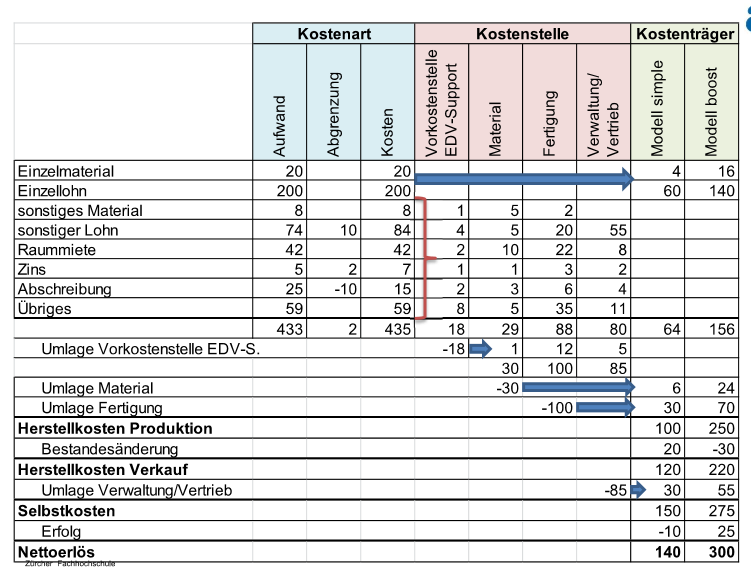
\includegraphics[width=0.3\textwidth]{Resources/Image/Vollkostenrechnung.png}
\caption{\label{fig:Vollkostenrechnung}Vollkostenrechnung.}
\end{figure}

\subsubsection{Ermittlung Zuschlagsätze}

\textbf{Zuschlagssatz=} ((Endstellenkosten(ESK) der Hauptkostenstelle)/Bezugsgrösse)*100
\\ \\

\textbf{Materialgemeinkostenzuschlagssatz=} ((Materialgemeinkosten)/Materialeinzelkosten)*100
\\ \\
\textbf{Fertigungsgemeinkostenzuschlagssatz=} ((Fertigungsgemeinkosten)/Fertigungseinzelkosten)*100
\\ \\

\textbf{Verwaltungskostenzuschlagssatz=} ((Verwaltungskosten)/Herstellkosten)*100\\ \\


\textbf{Vertriebsgemeinkostenzuschlagssatz=} ((Verwaltungskostengemeinkosten)/Herstellkosten)*100\\
Verwaltungskosten und Vertriebsgemeinkosten werden oft zusammengenommen.

\subsection{Teilkostenrechnung}
Beschränkt auf Einzelkosten:
\begin{itemize}
	\item Fixkosten
	\item Variable Kosten
	\begin{itemize}
		\item hängen von prod.Menge ab (z.B Materialeinzelkosten)
	\end{itemize}
	\item Deckungsbeitrag
	\begin{itemize}
		\item Wenn Verkaufspreis grösser als variable Kosten / Stk., Steht zur Deckung der fixen Kosten zur Verfügung.
	\end{itemize}
	\item Break-Even-Absatzmenge
\end{itemize}

\subsection{Break-Even-Analyse}
$Fixkosten(FK) + [var.Kosten(VK)/Stk. * Menge(x)] = Preis(P)/Stk * Menge(x) $\\
$Break-Even-Absatzmenge(x) = Fixkosten(FK) / Preis(P)/Stk. - Variable Kosten (VK)/Stk$ \\
$= Break-Even-Absatzmenge(x) = Fixkosten(FK) / Deckungsbeitrag/Stk.$\\
\begin{figure}[H]
\centering
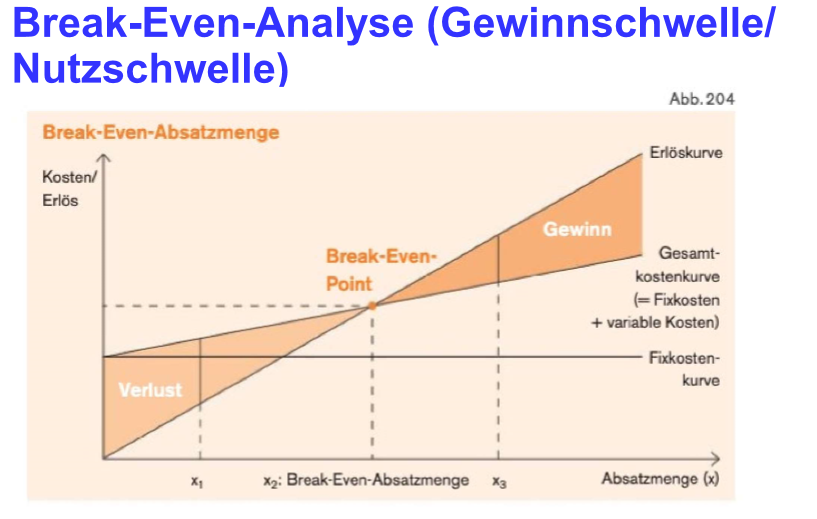
\includegraphics[width=0.3\textwidth]{Resources/Image/Break-Even-Absatzmenge.png}
\caption{\label{fig:Break-Even-Absatzmenge}Break-Even-Absatzmenge.}
\end{figure}

\paragraph{Ermittlung Nutzschwelle\\}
1. DB pro Stück = Stückerlös - variable Kosten\\
2. Nutzschwelle erreicht, wenn DB der verkauften Produkte alle Fixkosten decken\\

\textbf{Mengenmässige Nutzschwelle =} Fixkosten / DB pro Stk \\
\textbf{Wertmässige Nutzschwelle =} Mengenmässige Nutzschwelle * Verkaufspreis pro Stk.\\

\subsubsection{Deckungsbeitrag}
Verwendung in Preisgestaltung und Kostenüberwachung.\\

\subparagraph{Formel DB:\\}

Deckungsbeitrag pro Stück = Nettoerlös pro Stk(=Verk.Preis pro Stück) - variable Kosten pro Stk.\\


Reingewinn = Stück * BG(DB/stk) - GK \\

Bruttogewinn = DB pro Stück = Nettoerlös - aufwand / Verk.Menge \\
































































































































































































\end{document}